\documentclass[10pt,t]{beamer}

\usetheme[progressbar=frametitle]{metropolis}
\usepackage{appendixnumberbeamer}

\usepackage{booktabs}
\usepackage[scale=2]{ccicons}

\usepackage{pgfplots}
\usepgfplotslibrary{dateplot}

\usepackage{xspace}
\newcommand{\themename}{\textbf{\textsc{metropolis}}\xspace}
\newcommand{\titleskip}{15pt}
\newcommand{\secondskip}{15pt}

\usepackage{graphicx} %Loading the package
\graphicspath{{figures/}} %Setting the graphicspath

\usepackage{marvosym} 	% bold rightarrow
\usepackage{xcolor}		% colored text
\usepackage{hyperref}   % insert hyperlinks
\usepackage{appendixnumberbeamer} % to identify start of appendix

\newcommand\setItemnumber[1]{\setcounter{enumi}{\numexpr#1-1\relax}} %set item number enumerate

\title{Machine learning the parton distribution functions}
\subtitle{Generalizing the methodology}

\date{\vspace{-0.3cm} First year PhD workshop \\ 22 September 2020}
\author{Roy Stegeman}
\institute{University of Milan and INFN Milan}

\titlegraphic{\vspace*{145pt}
		
\includegraphics[height=1.1cm]{LOGO-ERC.jpg} \hspace{1.0cm}
		
\includegraphics[height=1.1cm]{n3pdflogo_noback.png} \hspace{1.0cm}
		\includegraphics[height=1.1cm]{Logo_Università_degli_Studi_di_Milano(not_mandatory).png}
		
\includegraphics[height=1.1cm]{INFN_logo.png}
        \vspace{0.1cm} \\
		\centering{ \fontsize{6.0pt}{6.0pt}\selectfont This project has received funding from the European Union’s Horizon 2020 research and innovation programme under grant agreement No 740006.}
	}

\begin{document}

\setbeamercolor{background canvas}{bg=white}
\maketitle

% Proton is made out of partons (quarsk + gluons) which contain a colour charge resulting in an interaction called the strong interaction. The theory describing this interaction is called QCD.

% Coupling constant depends on the energy scale of the interaction. 

\begin{frame}{Outline}

\vspace*{\titleskip}

	\begin{enumerate}
		\item {\textbf{Motivation}}
		\begin{itemize}
			\item What are parton distribution functions (PDFs)?
			\item Why do we want to determine them?
		\end{itemize}
		
		\item {\textbf{Current Methodology}}
		\begin{itemize}
			\item The Machine Learning problem
			\item The NNPDF methodology
		\end{itemize}

		\item {\textbf{Towards a new methodology}}
		\begin{itemize}
			\item Generalized architecture
		\end{itemize}
	
		\item{\textbf{Outlook}}
		\begin{itemize}
		\item The extrapolation region
		\end{itemize}
		
	\end{enumerate}
	
\end{frame}


\section{Motivation}

\begin{frame}{Quantum Chromodynamics}

\vspace*{\titleskip}

\begin{columns}[T,onlytextwidth]
	\column{0.70\textwidth}
	\begin{itemize}

		\item The theory of the {strong interaction} is called {Quantum Chromodynamics (QCD)}
		
		\begin{itemize}
		\item Binds quarks to form hadrons 
		\end{itemize}

		\item Quantum field theory where quarks and gluons (partons) are the fundamental fields
		
		\item QCD cannot be solved exactly, but we can approximate using perturbative expansion
		
%		\item Quarks carry fractional electric charge
%		\item Quarks posses a property called \textbf{colour  charge}
	
	\end{itemize}
	\column{0.05\textwidth}
	\column{0.25\textwidth}
	\vspace*{0pt}
	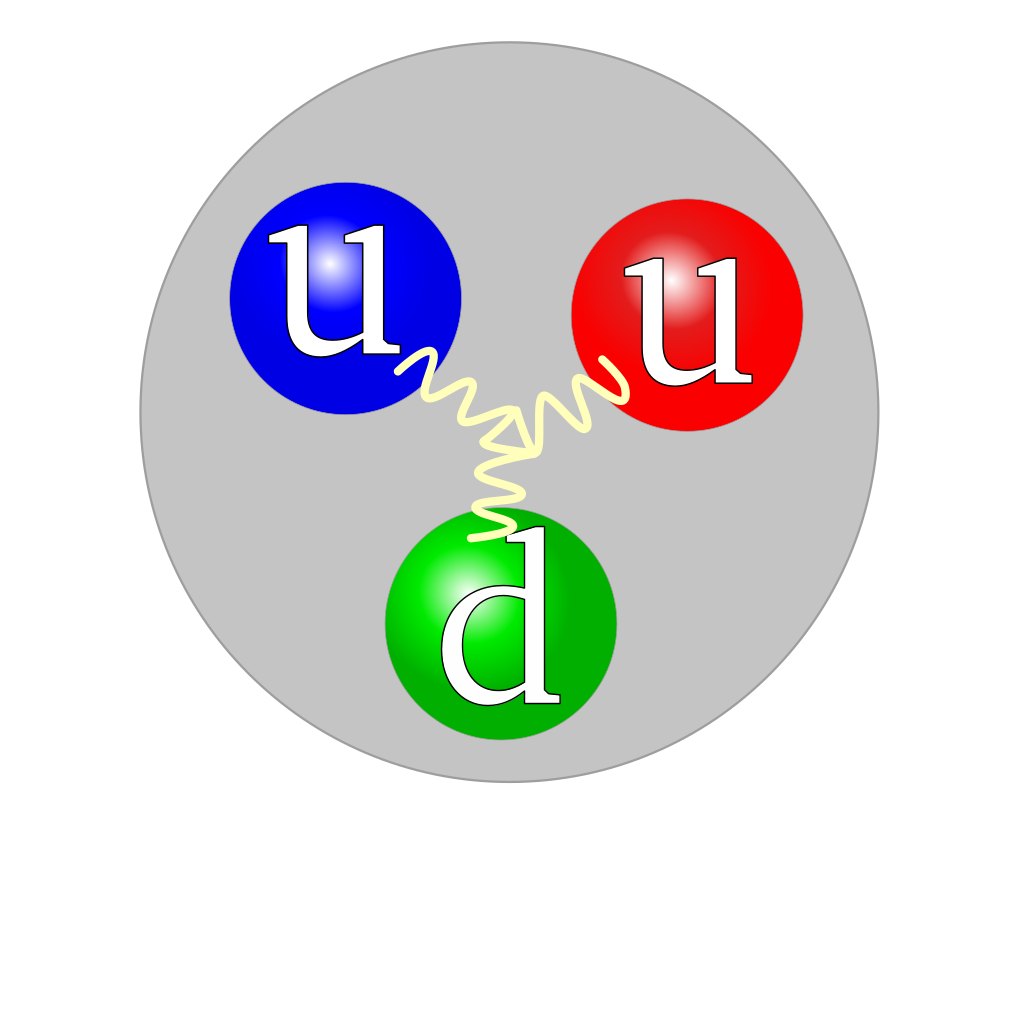
\includegraphics[width=0.95\textwidth]{proton_structure_uud}
\end{columns}


\end{frame}

%%=============================================================

\begin{frame}{Quantum Chromodynamics}

\vspace*{\titleskip}

\begin{itemize}
	\item The expansion is in term of the strong coupling constant $\alpha_s$
	
	\begin{itemize}
	\item The strength of the interaction is given by $\alpha_s$
	\end{itemize}

%	\item The strength of the interaction is described by the strong coupling constant $\alpha_s$
	
	\item $\alpha_s$ decreases as the  energy increases
	
	\item In the high energy limit we can expand in $\alpha_s$
	
\end{itemize}

\end{frame}

%=============================================================


%\begin{frame}{Parton distribution functions (PDFs)}
%
%\vspace*{\titleskip}
%
%\begin{columns}[T,onlytextwidth]
%	\column{0.70\textwidth}
%	\begin{itemize}
%	
%	\item PDFs describe the partonic substructure of hadrons
%
%	\item PDFs are needed to provide a theoretical prediction for particle physics experiments
%	
%	\end{itemize}
%	\column{0.05\textwidth}
%	\column{0.25\textwidth}
%	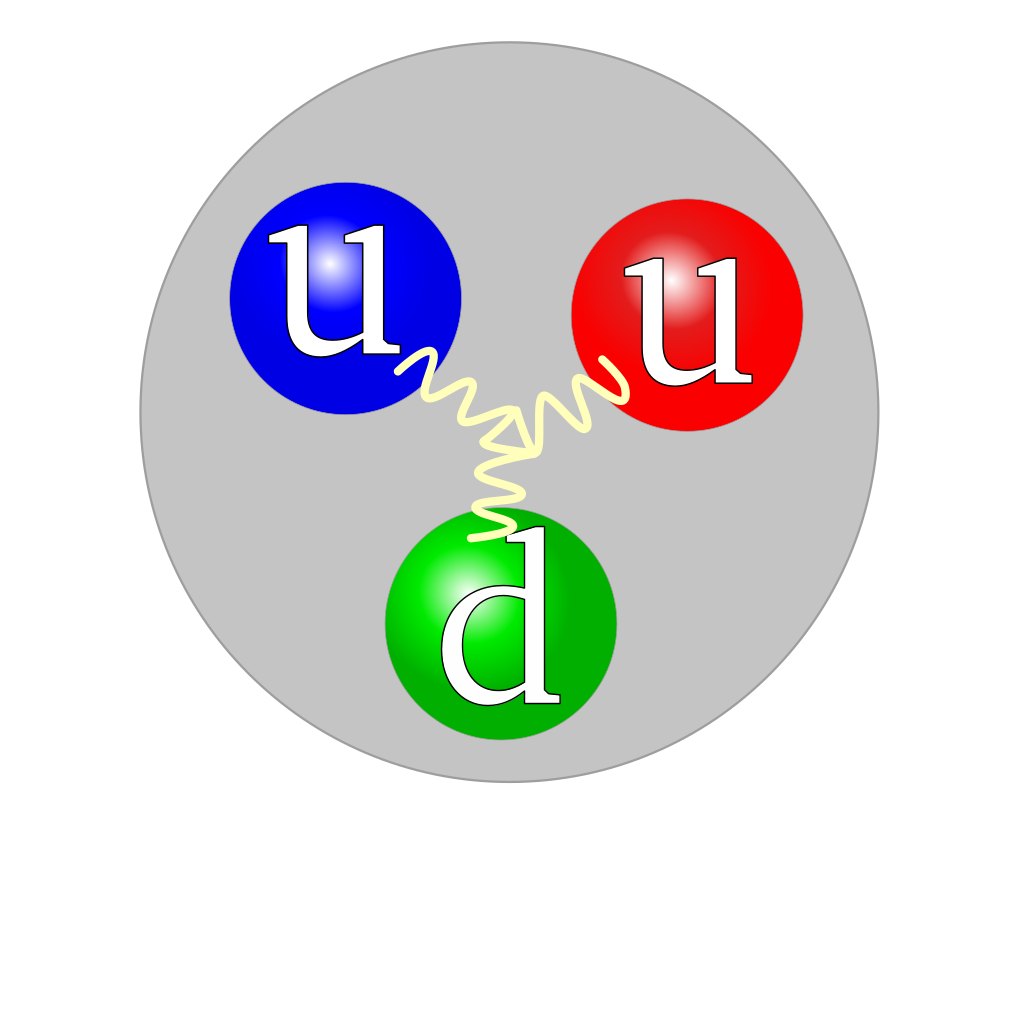
\includegraphics[width=0.95\textwidth]{proton_structure_uud}
%\end{columns}
%
%
%\end{frame}

\begin{frame}{Parton distribution functions (PDFs)}

\vspace*{\titleskip}

\begin{itemize}
	\item PDFs are required to provide theoretical predictions	

	\item Hadron collisions are factored into a 'hard part' $\hat{\sigma}$ and a normalization provided by the PDFs	
	
	\item PDFs provide the probablity of extracting a parton of a certain type (up, down, ..) from a hadron  	
	
%	\item We cannot calculate PDFs
	
%	\item PDFs are a universal property of a hadron
	
%	\item We do not have reasons to assume a functional form of the PDFs	
	
\end{itemize}

\begin{center}

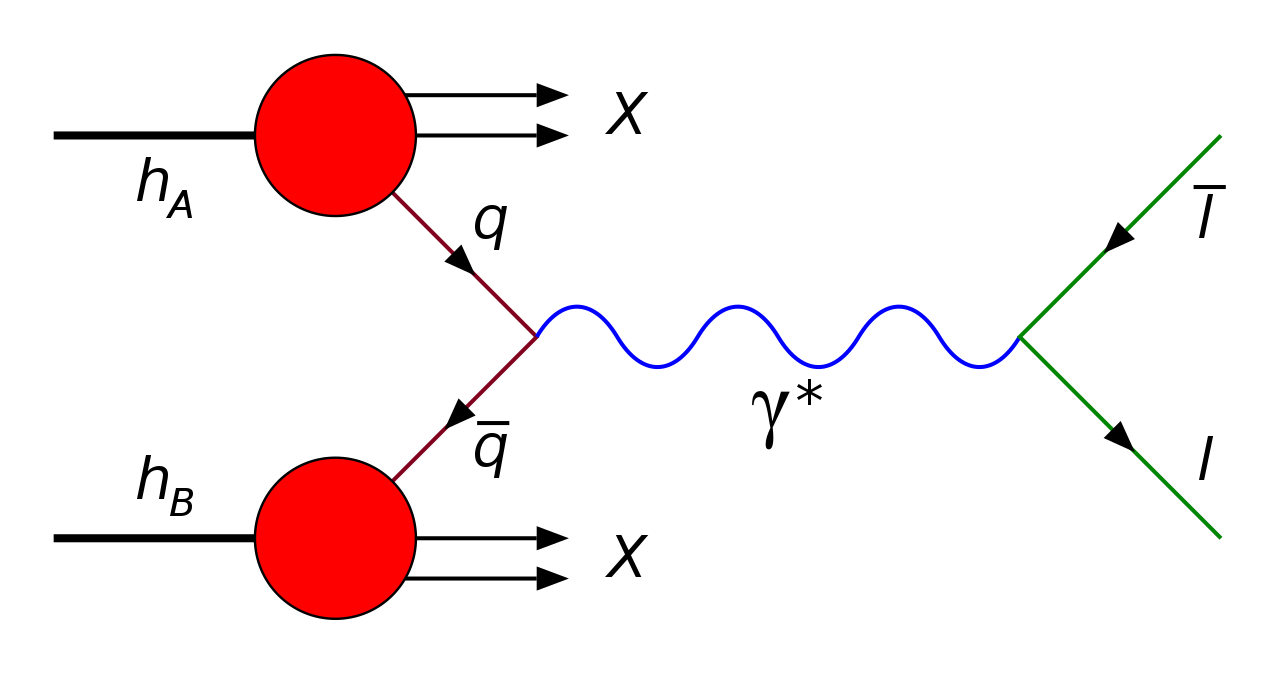
\includegraphics[width=0.5\textwidth]{Drell-Yan}

\vspace{-0.5cm}
$$ \overbrace{\sigma_X}^{\text{observable}}=\sum_{a, b} \int d x_{1} d x_{2} \overbrace{ f_{a / h_{A}}\left(x_{1}\right) f_{b / h_{B}}\left(x_{2}\right)}^{\text{PDFs}} \overbrace{ \hat{\sigma}_{a b \rightarrow X}}^{\text{theory}} $$
%$$ \overbrace{\sigma_X\left(s,\mu^2\right)}^{\text{experiment}}=\sum_{a, b} \int_{0}^{1} d x_{1} d x_{2} \overbrace{ f_{a / h_{A}}\left(x_{1}, \mu^{2}\right) f_{b / h_{B}}\left(x_{2}, \mu^{2}\right)}^{\text{PDFs}} \overbrace{ \hat{\sigma}_{a b \rightarrow X}\left(\mu^{2}\right)}^{\text{theory}} $$

\end{center}


\end{frame}

%=============================================================

%\begin{frame}{Parton distribution functions}
%
%\vspace*{\titleskip}
%An accurate determination of PDFs is needed to determine the expected observables for an experiment.  
%\vspace*{\secondskip}
%
%\begin{center}
%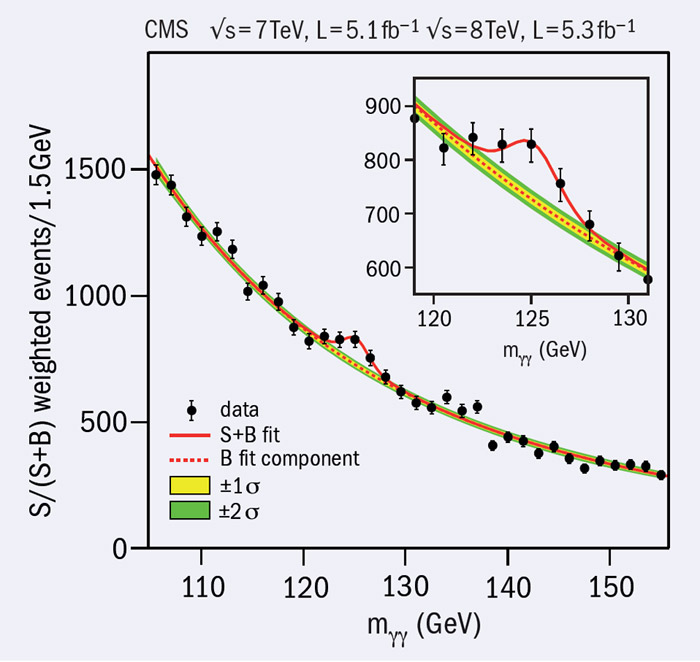
\includegraphics[width=0.5\textwidth]{Higgs_measurement}
%\end{center}
%
%\end{frame}

%=============================================================

\section{Current Methodology}

\begin{frame}{The NNPDF collaboration}

\vspace*{\titleskip}

\begin{center}

\includegraphics[width=0.4\textwidth]{nnpdflogo_noback}
\end{center}

\vspace*{\secondskip}

\begin{itemize}
	\item NNPDF provides a PDF determination using Neural Networks
\end{itemize}

\end{frame}

%=============================================================

\begin{frame}{The fitting problem}

\vspace*{\titleskip}

\begin{itemize}
	
\item First fitting attempt: $f_i=A_ix^{\alpha_i}(1-x)^{\beta_i}$
	
\item Based on arguments in the limits $x\rightarrow 0$ and $x \rightarrow 1$

%\item PDFs are scale dependent 

\item Assuming a functional form leads to underestimation of PDF uncertainties

%\item This can be overcome by using a neural network
	
\end{itemize}

\vspace*{\secondskip}

\begin{center}
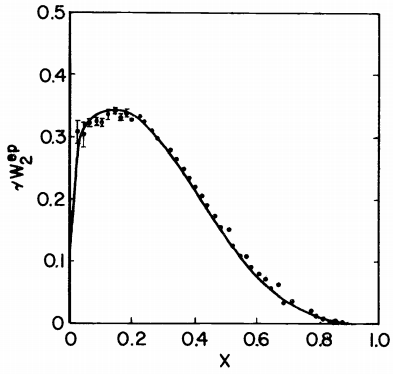
\includegraphics[width=0.3\textwidth]{first_pdf}\\
{\small \text{McElhaney, Tuan (1973)}}
\end{center}

\end{frame}

%=============================================================

\begin{frame}{The NNPDF methodology}

\vspace*{\titleskip}

\begin{itemize}
\item Using a Neural Network reduces bias from the functional form
\begin{itemize}
\item $f_i=\text{A}_ix^{\alpha_i}(1-x)^{\beta_i}\text{NN}_i(x,\log x)$
\end{itemize}
\item Monte Carlo set of PDFs
\begin{itemize}
\item As physicists, we believe data is Gaussian: $X\sim \mathcal{N}(\mu, \sigma^2)$
\item Sample $\mathcal{N}(\mu, \sigma^2)$ to create pseudo data sets
\item Expectation values are calculated for properties of interest
\end{itemize}
%\item Minimization using gradient descent 
%\item Stopping based on training/validation data
\end{itemize}

\vspace*{\secondskip}

\begin{columns}[T,onlytextwidth]
	\column{0.475\textwidth}
	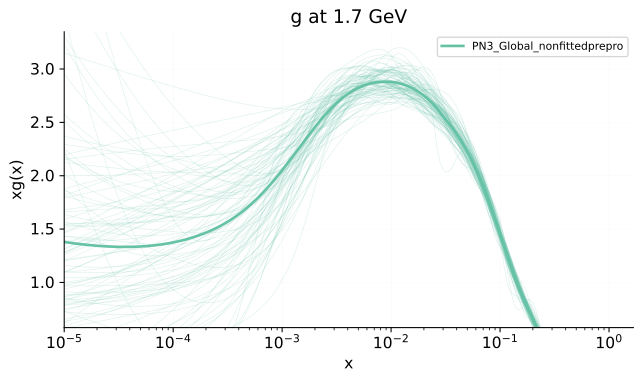
\includegraphics[width=\textwidth]{pdfreplicas}
	\column{0.05\textwidth}
	\column{0.475\textwidth}
	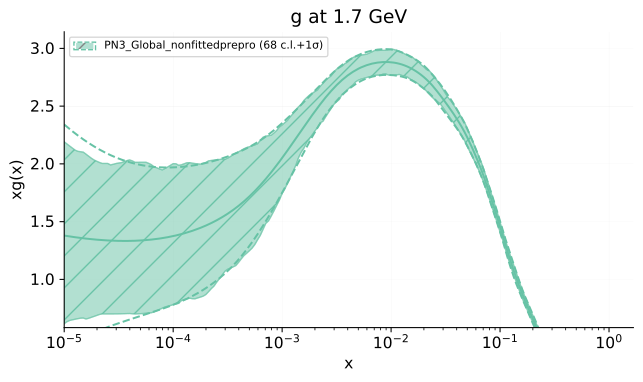
\includegraphics[width=\textwidth]{pdfplot}
\end{columns}

\end{frame}

%=============================================================

\section{Towards a new methodology}


\begin{frame}{Prejudice}

\vspace*{\titleskip}
The methodology is still not completely free of prejudice 
\begin{itemize}
\item $f_i=\text{A}_ix^{\alpha_i}(1-x)^{\beta_i}\text{NN}_i(x,\log x)$
\end{itemize}

If preprocessing is removed, we observe freezing at small-x:
\vspace*{\secondskip}

\begin{center}
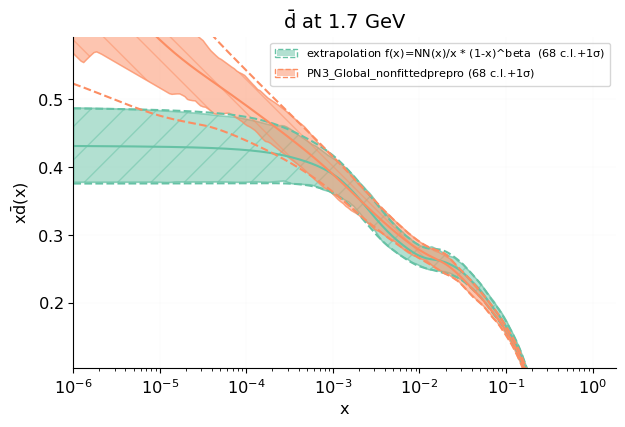
\includegraphics[height=0.3\textwidth]{flatdbar}
\end{center}

\end{frame}

%=============================================================

\begin{frame}{Feature Scaling}

\vspace*{\titleskip}

Solution:
\begin{enumerate}
\item<1-|alert@1-3> Scale the input xgrid such that it is homogeneously distributed
\item<1-|alert@4> Select one in $n$ points  
\item<1-|alert@5> Provide a monotonically increasing interpolation
\end{enumerate}

\only<1-5>{{ Result: $f_i=\text{A}_i \text{NN}_i(x')$}}
\only<6>{\alert{ Result: $f_i=\text{A}_i \text{NN}_i(x')$}}
\only<7>{\alert{ Result: $f_i=\text{A}_i \left(\text{NN}_i(x')-\text{NN}_i(1)\right)$}}

% figures of xgrid histogram, or maybe simple example of 1D grid of points
\begin{center}
\only<1>{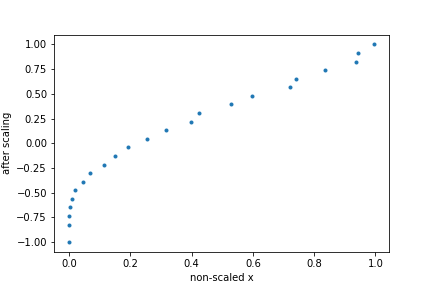
\includegraphics[height=0.3\textwidth]{feature_scaling_1}}
\only<2>{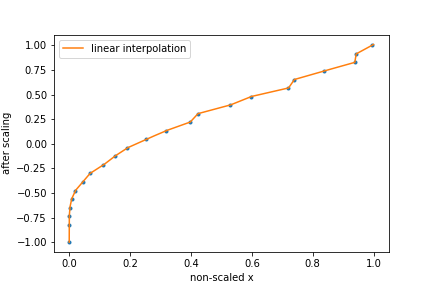
\includegraphics[height=0.3\textwidth]{feature_scaling_2}}
\only<3>{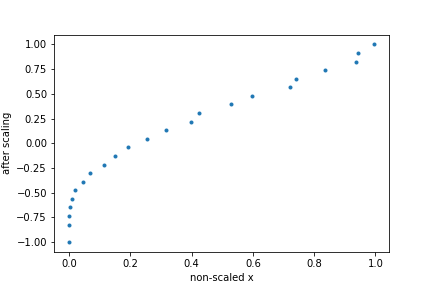
\includegraphics[height=0.3\textwidth]{feature_scaling_1}}
\only<4>{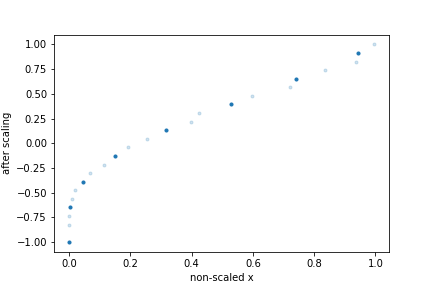
\includegraphics[height=0.3\textwidth]{feature_scaling_3}}
\only<5-6>{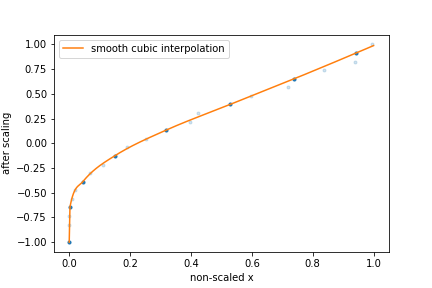
\includegraphics[height=0.3\textwidth]{feature_scaling_4}}
\only<7>{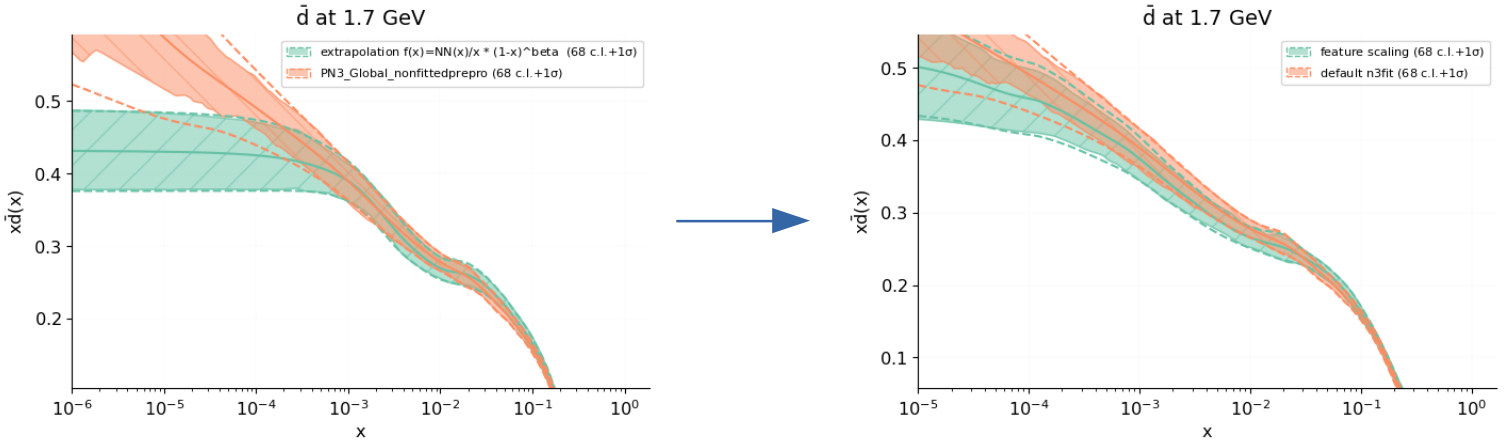
\includegraphics[height=0.3\textwidth]{flat_to_feature}
}
\end{center}

\end{frame}


%=============================================================
\section{Outlook}
\begin{frame}{ The extrapolation region}

\vspace*{\titleskip}

\begin{itemize}
%\item We lost the prediction for the extrapolation region
\item Use Gaussian Process Regression to fit observables + uncertainty

\begin{itemize}
\item Important: as physicists, we believe data is Gaussian
\end{itemize}
\item Generate observables in the extrapolation region
\item Include this Gaussian pseudodata in the NNPDF fit
%\item Machine Learning goes where theory or experiments can't
\end{itemize}

\vspace*{\secondskip}

%\begin{columns}[T,onlytextwidth]
%	\column{0.475\textwidth}
%	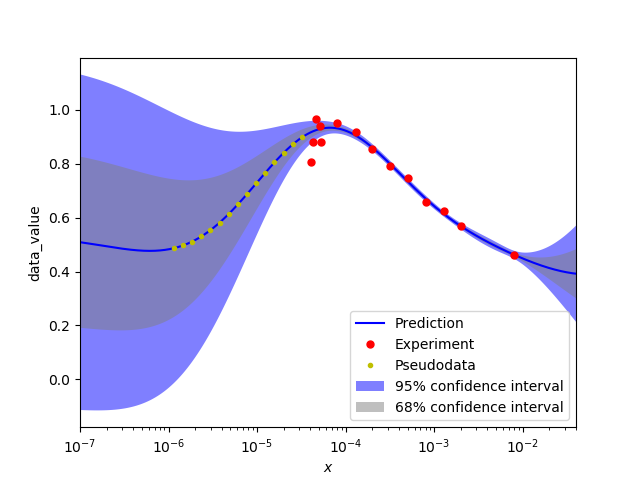
\includegraphics[width=\textwidth]{GP}							\column{0.05\textwidth}
%	\column{0.475\textwidth}
%	\vspace{0.7cm}
%	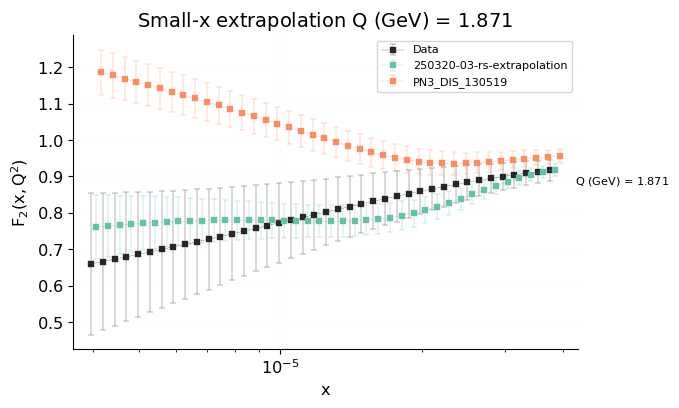
\includegraphics[width=\textwidth]{preproc_dominates_smallx}
%\end{columns}

\begin{center}
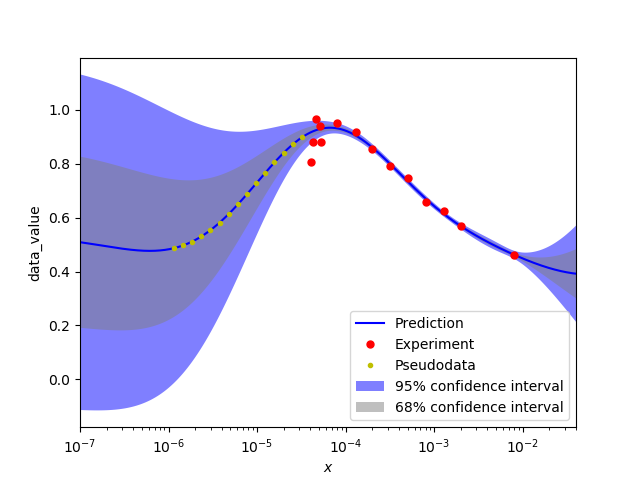
\includegraphics[width=0.5\textwidth]{GP}
\end{center}


\end{frame}

%=============================================================


%\section{Conclusions}
%
%
%\begin{frame}{Conclusions}
%
%\vspace*{\titleskip}
%
%Conclusions:
%	\begin{itemize}
%		\item PDFs are needed to make the connection between theory and experiment
%		
%		\item Neural Network reduces bias in PDF determination
%		
%		\item We have shown a method to generalize the methodology even further
%				
%	\end{itemize}
%	
%Outlook: 
%\begin{itemize}
%\item Provide a prediction in the extrapolation region
%\end{itemize}
%
%
%\end{frame}

%=============================================================

{
\setbeamercolor{background canvas}{bg=mDarkTeal}
\begin{frame}[plain,noframenumbering]
\vspace{0.5\textheight}
\centering \Large \color{white} \textbf{Thank you!}
\end{frame}
}

\begin{frame}[plain, noframenumbering]{n3fit code}

\vspace*{\titleskip}
\begin{center}
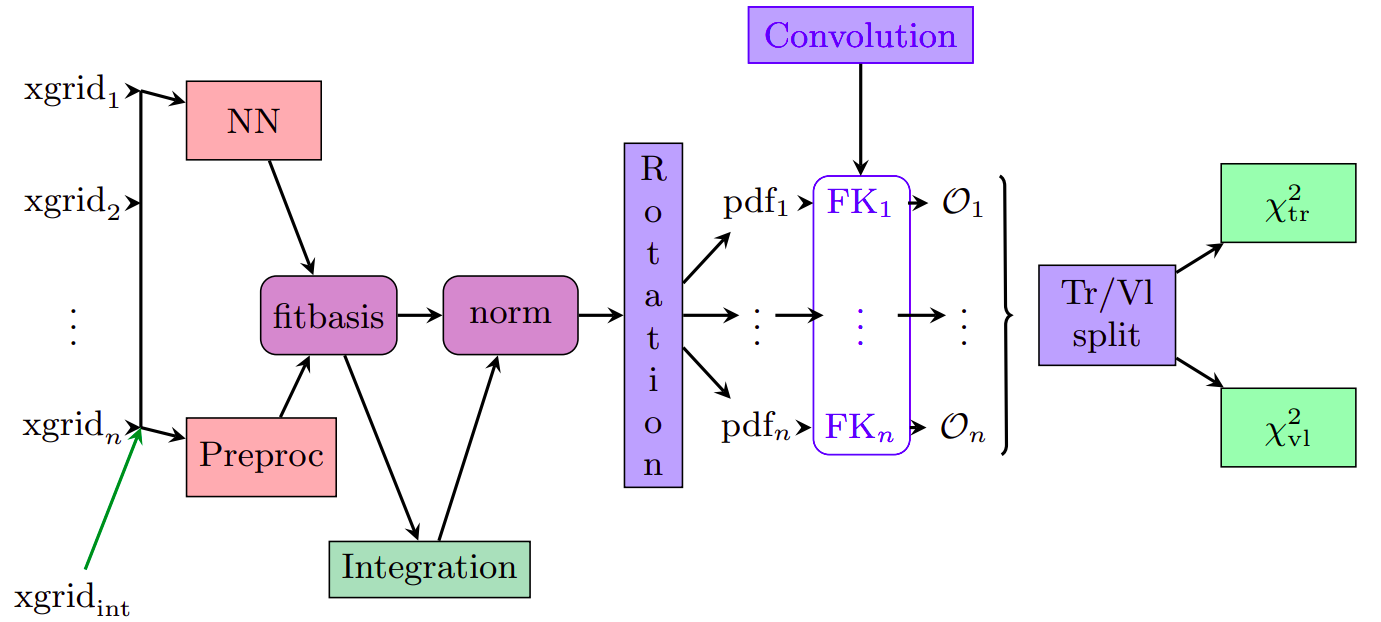
\includegraphics[width=0.9\textwidth]{n3fit_architecture}
\end{center}

\end{frame}

\begin{frame}[plain, noframenumbering]{patience algorithm}

\vspace*{\titleskip}
\begin{center}
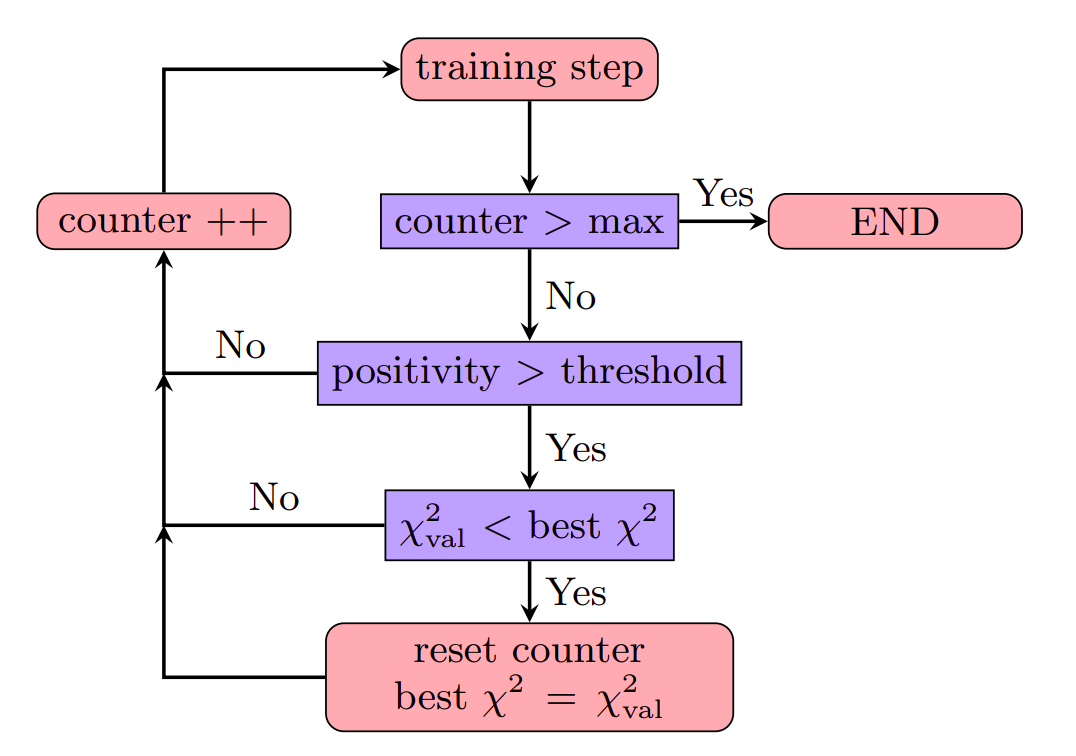
\includegraphics[width=0.8\textwidth]{patience}
\end{center}

\end{frame}


\end{document}
